%
%%%%%%%%%%%%%%%%%%%%%
\section{Diagrammes}
%%%%%%%%%%%%%%%%%%%%%
%
\subsection{Cas d'utilisation}
%
Ce diagramme présente les interactions entre l'utilisateur et le programme à travers l'interface graphique.
%
\begin{center}
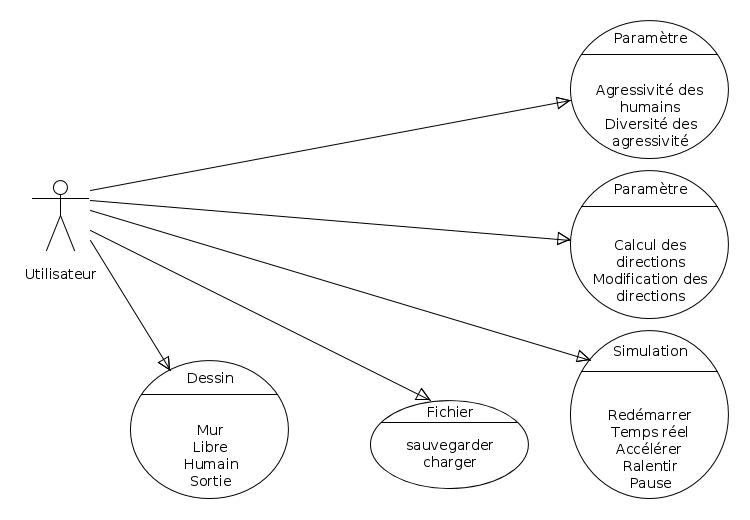
\includegraphics[scale=0.65]{./illustration/casDutilisation}
\end{center}
%

%
\newpage
%
\subsection{diagramme d'inclusion 2.0}
%
Ce diagramme présente les classes de SimFoule, indique l'inclusion des fichiers. La coloration indique les répertoires.
%
\begin{center}
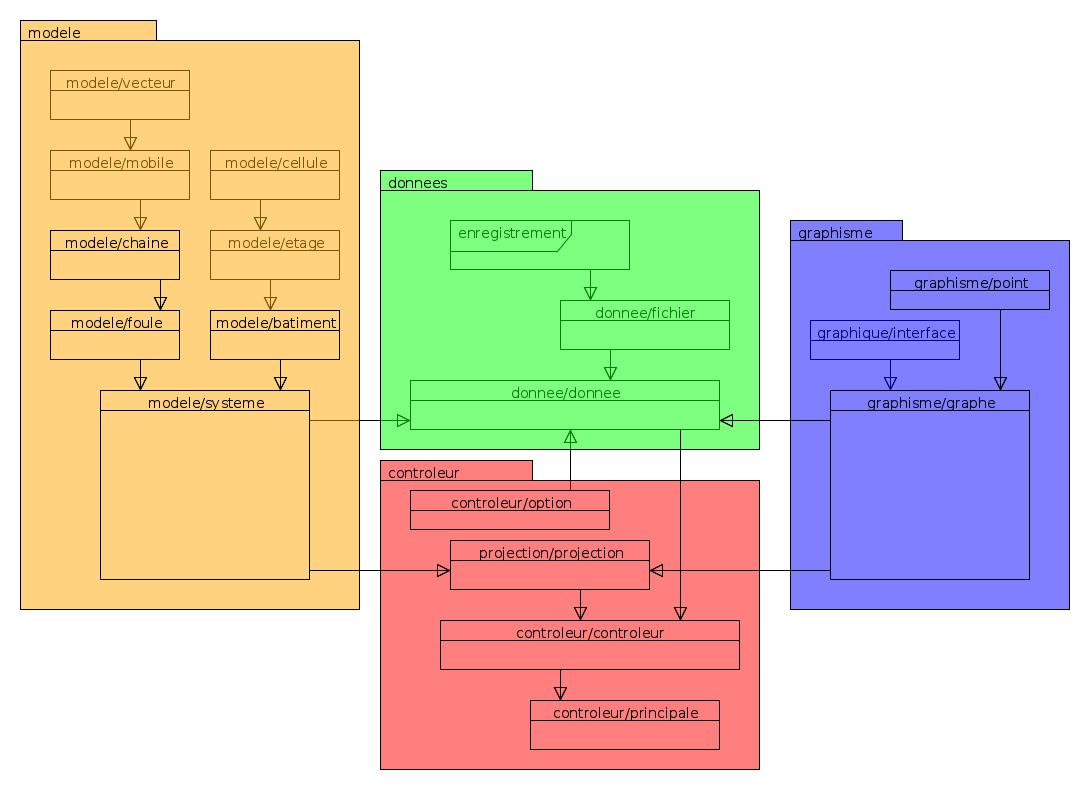
\includegraphics[scale=0.45]{./illustration/classesSimFoule}
\end{center}
%
\begin{comment}
\subsection{diagramme de classes}
%
Ce diagramme présente les classes de SimFoule et indique l'inclusion des fichiers.
%
\begin{center}
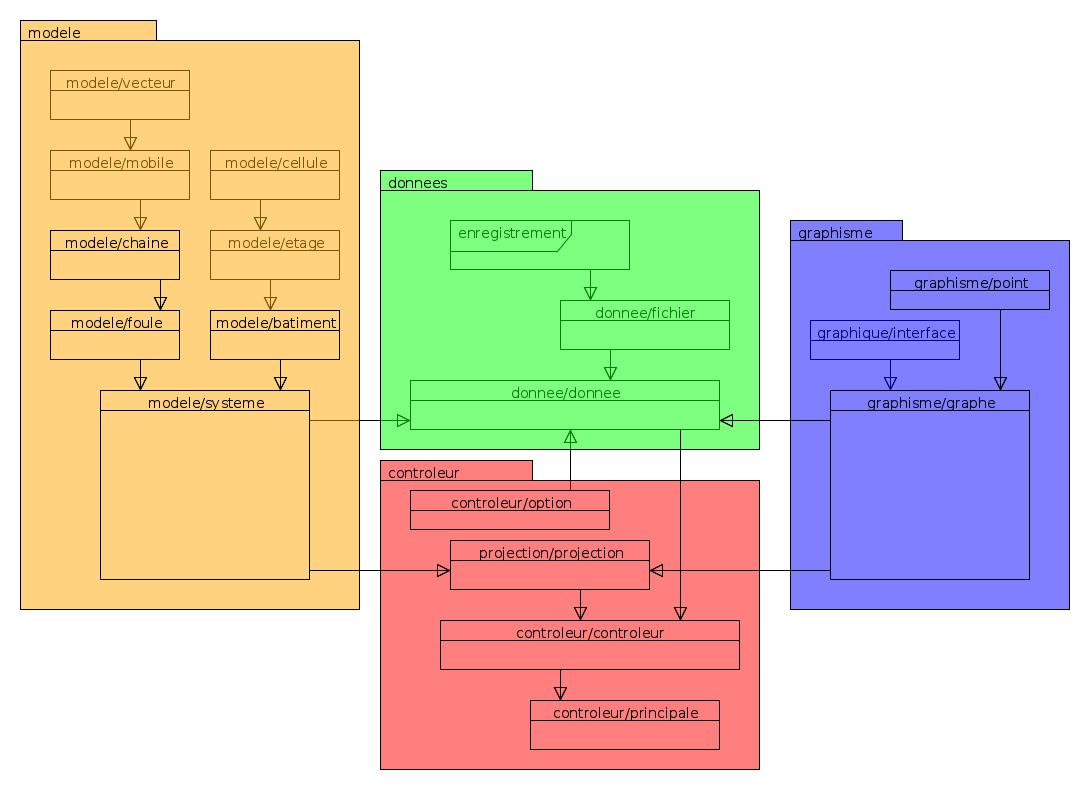
\includegraphics[scale=0.45]{./illustration/classesSimFoule}
\end{center}
\end{comment}
%
\newpage
%
\subsection{diagrammes de séquences}
%
%
\subsubsection{Principale 2.0}
%\begin{center}
%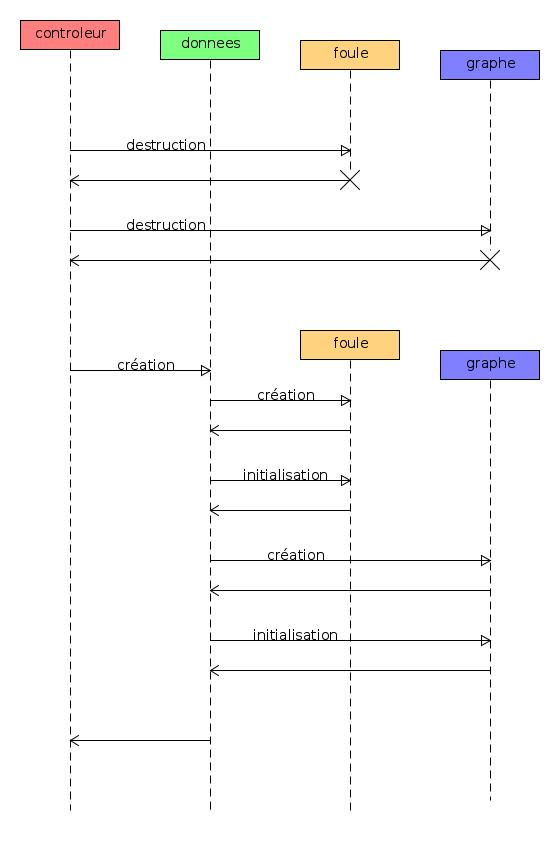
\includegraphics[scale=0.51]{./illustration/sequenceReinitialisation}
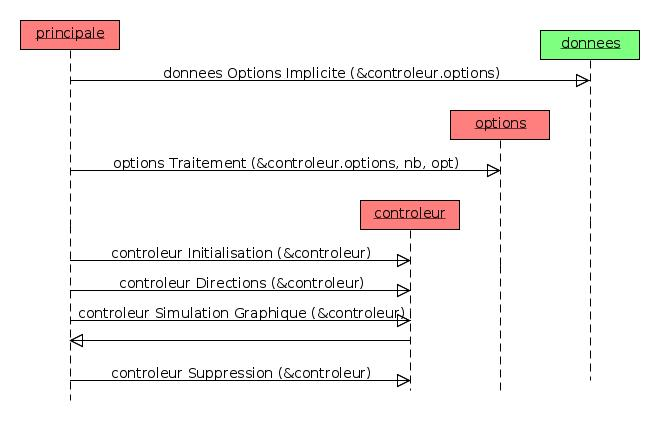
\includegraphics[width=.95\textwidth]{./illustration/sequenceInitialisationPrincipale}

\vspace{.91cm}
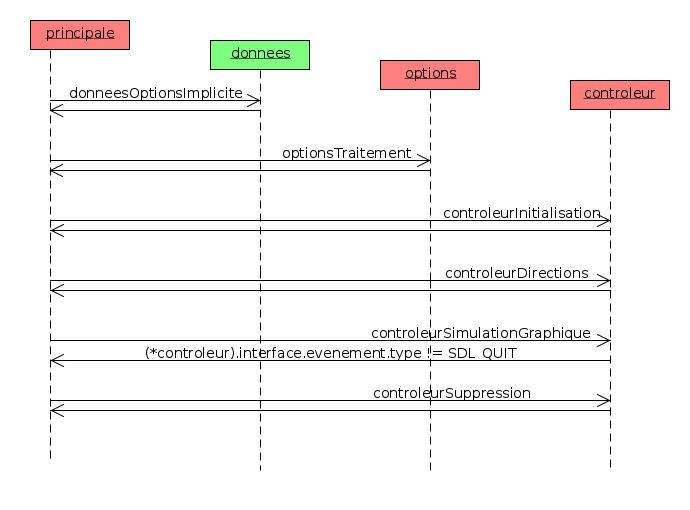
\includegraphics[width=.95\textwidth]{./illustration/sequencePrincipale2}
%\end{center}
%
\subsubsection{Simulation graphique 2.0}
%\begin{center}
%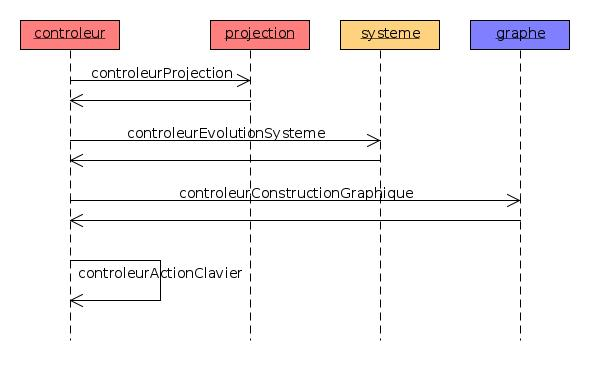
\includegraphics[scale=0.51]{./illustration/sequenceControleur}
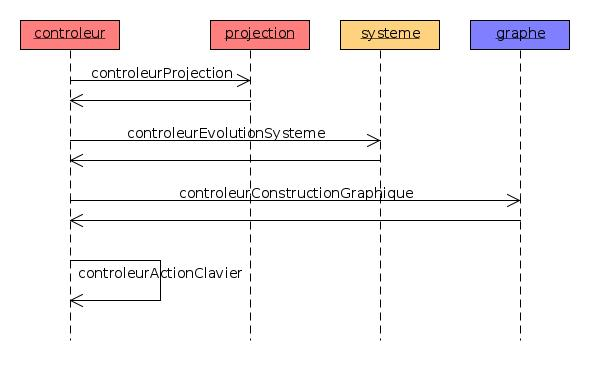
\includegraphics[width=.95\textwidth]{./illustration/sequenceControleur}
%\end{center}
%
\newpage
%
\subsubsection{Réinitialisation 2.0}
%\begin{center}
%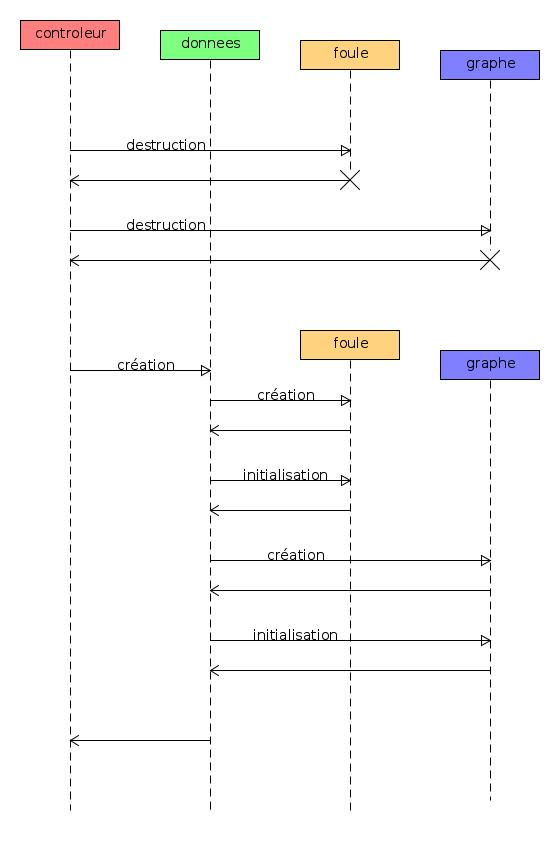
\includegraphics[scale=0.51]{./illustration/sequenceReinitialisation}
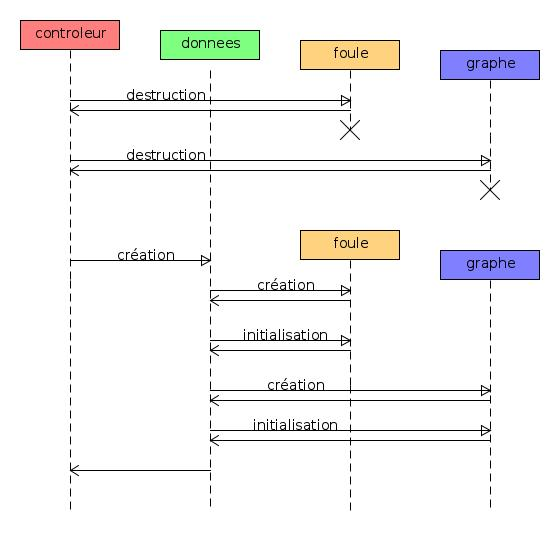
\includegraphics[width=.75\textwidth]{./illustration/sequenceReinitialisation2}
%\end{center}

%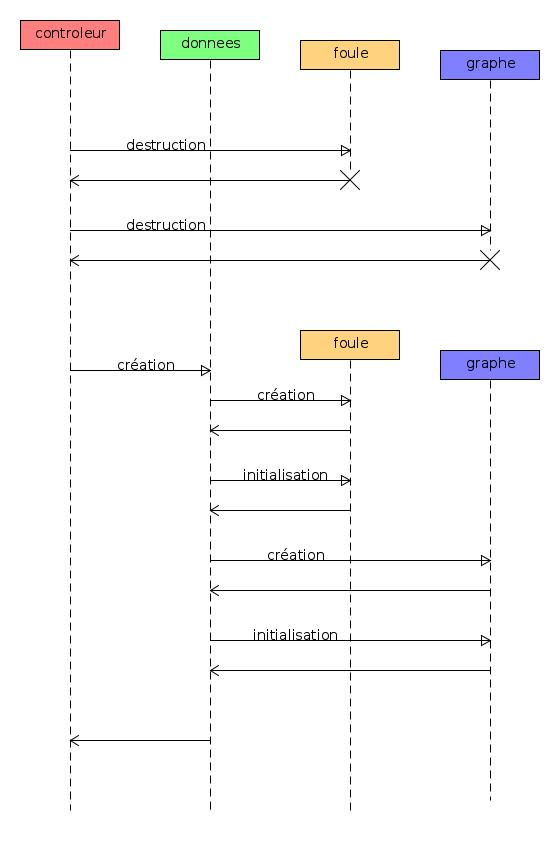
\includegraphics[scale=0.51]{./illustration/sequenceReinitialisation}
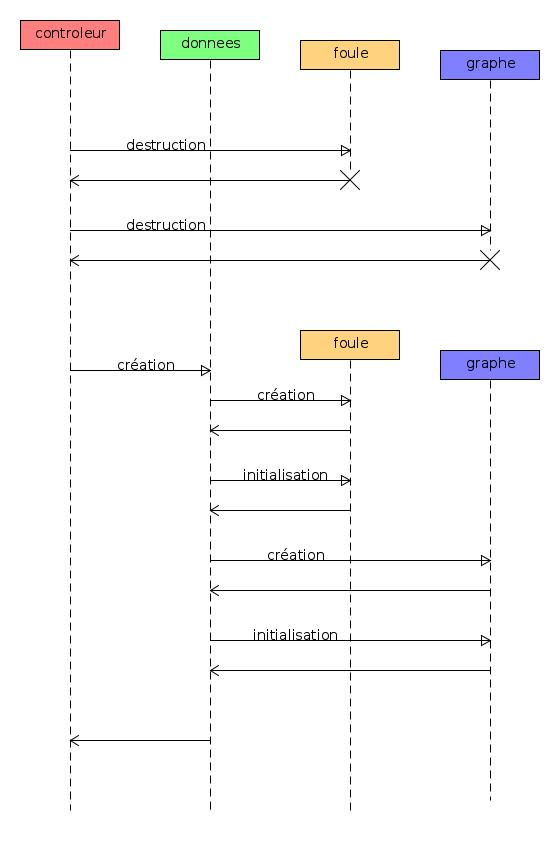
\includegraphics[width=.35\textwidth]{./illustration/sequenceReinitialisation}
%\end{center}
%
\newpage
%
\subsubsection{Construction 2.2}
%\begin{center}
%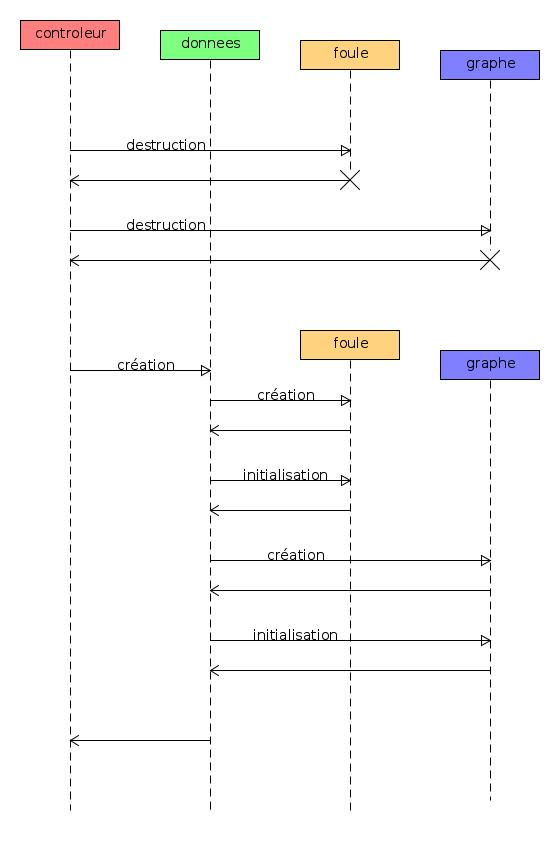
\includegraphics[scale=0.51]{./illustration/sequenceReinitialisation}
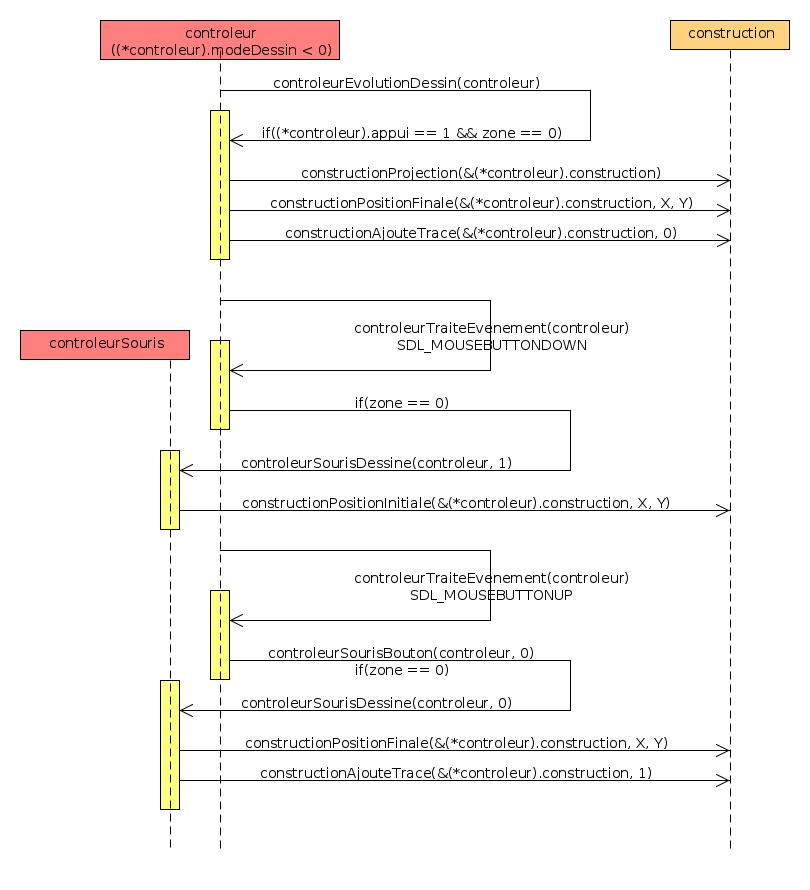
\includegraphics[width=1.05\textwidth]{./illustration/sequenceControleurConstruction}
%\end{center}
%
\newpage
%
\subsubsection{Construction 2.2}
%%%%%%%%%%%%%%%%%%%%%%%%%%%%%%%%%%%%%%%%%%%%
%%%%%%%%%%%%%%%%%%%%%%%%%%%%%%%%%%%%%%%%%%%%
%\begin{itemize}[leftmargin=2cm]
%\item \texttt{gras} : texte
%\end{itemize}



%%%%%%%%%%%%%%%%%%%%%%%%%%%%%%%%%%%%%%%%%%%%%%%%%%%%%%%%%%%%%%%%%%%%%%%%%%%%%%%%%%%%%
